%%%%%%%%%%%%%%%%%%%%%% Props %%%%%%%%%%%%%%%%%%%%%%
\documentclass{article}

\usepackage[french]{babel}
\usepackage[utf8]{inputenc}
\usepackage[T1]{fontenc}
\usepackage{graphicx}
\usepackage{fancyhdr}
\usepackage{eurosym}
\usepackage{color}
\usepackage{soul}
\usepackage{listings}
\usepackage{enumitem}
\usepackage{enumerate}

\pagestyle{fancy}
\lhead{Cahier des charges}
\chead{Deadly Science}
\rhead{Custos Carceris}

\definecolor{mygreen}{rgb}{0,0.6,0}
\definecolor{mygray}{rgb}{0.5,0.5,0.5}
\definecolor{mymauve}{rgb}{0.58,0,0.82}

\lstset{ 
  commentstyle=\color{mygreen},
  keywordstyle=\color{blue},       % keyword style
  numberstyle=\tiny\color{mygray}, % the style that is used for the line-numbers
  rulecolor=\color{black},         % if not set, the frame-color may be changed on line-breaks within not-black text (e.g. comments (green here))
  stringstyle=\color{mymauve},     % string literal style
  language=[Sharp]C,                 % the language of the code
  backgroundcolor=\color{white},   % choose the background color; you must add \usepackage{color} or \usepackage{xcolor}; should come as last argument
  basicstyle=\footnotesize,        % the size of the fonts that are used for the code
  breakatwhitespace=true,         % sets if automatic breaks should only happen at whitespace
  breaklines=true,
  extendedchars=true,              % lets you use non-ASCII characters; for 8-bits encodings only, does not work with UTF-8
  frame=single,	                   % adds a frame around the code
  tabsize=2,	                   % sets default tabsize to 2 spaces
  showstringspaces=false,
  numbers=left,
}

\begin{document}


%%%%%%%%%%%%%%%%%%%%%% Titre %%%%%%%%%%%%%%%%%%%%%%
\begin{titlepage}
	\centering
	{\scshape\LARGE Custos Carceris\par}
	\vspace{1cm}
	{\scshape\Large Seconde soutenance \par}
	\vspace{1.5cm}
	{\huge\bfseries Deadly Science\par}
	\vspace{2cm}
	
\includegraphics[width=0.5\textwidth]{logo.png}\par\vspace{1cm}
	{\Large\itshape Léandre Perrot\par}
	{\Large\itshape Yann Boudry\par}
	{\Large\itshape Steve Suissa\par}
	{\Large\itshape Célian Raimbault\par}
	\vfill
	Un projet EPITA
	\vfill
	{\large \today\par}
\end{titlepage}



\newpage
\tableofcontents


%%%%%%%%%%%%%%%%%%%%% Intro %%%%%%%%%%%%%%%%%%%%%%

\newpage
\section{Introduction}

%%%%%%%%%%%%%%% TODO : Mettre a jour
Le jeu a grandement avancé depuis le retour du cahier des charges : le réseau est quasiment entièrement fonctionnel, pareil pour la caméra, le site avance petit à petit, la génération est presque fini et certaines musiques ont été composées. Globalement, le jeu est quasiment jouable.
\begin{table}[!h]
\centering
\caption{Avancement}
\begin{tabular}{|l|l|l|}

\hline
%%%%%%%%%%%%%%% TODO : Mettre a jour
Tâches $\backslash$Soutenances & Attendu & Réalité \\ \hline
Camera & 50\% & 75\% \\ \hline
G Joueur & 30\% & 50\% \\ \hline
G Jeu & 30\% & 30\% \\ \hline
Reseau & 50\% & 75\% \\ \hline
Map Const & 30\% & 30\% \\ \hline
Menu & 15\% & 70\% \\ \hline
Chrono/GUI & 30\% & 30\% \\ \hline
Site TXT & 0\% & 30\% \\ \hline
Site E & 0\% & 0\% \\ \hline
Map Gen & 0\% & 50\% \\ \hline
Musique & 0\% & 25\% \\ \hline
Sons & 0\% & 10\% \\ \hline

\end{tabular}
\end{table}
 
\newpage
\section{Réalisations}

%%%%%%%%%%%%%%%%%% TODO : Introduction


%%%%%%%%%%%%%%%%%%%%% Celian %%%%%%%%%%%%%%%%%%%%%%%%%%
\newpage
\subsection{Célian}

Les modifications que j'ai apporté pour cette soutenance ont principalement pour but de porter le jeu en réseau, j'entends par cela uniquement la phase de jeu. Je me suis plus précisement occupé de synchroniser certaines variables entre les joueurs comme leur status, j'ai également géré l'envoie de plusieurs évenements comme le début / la fin du jeu et dernièrement j'ai ajouté un peu de son au jeu pour le rendre un peu plus vivant.

\paragraph{Phases et status}

\subparagraph{Implémentation locale}

Rappel : Le jeu est composé de deux phases, la première où les joueurs doivent trouver les sérums et la seconde où les joueurs qui n'ont pas réussi à trouver de sérums doivent se venger et empécher les joueurs guéris de gagner en les touchant.

Un joueur peut avoir 4 status différents, pour l'instant 3 d'entre eux sont implémentés correctement :

\begin{itemize}
\item Infécté : Au début du jeu, il faut trouver un sérum pour passer en guéris et non en mode revanche
\item Guéris : Ce joueur à presque gagné, il doit éviter les joueurs encore infectés - en mode revanche - pour gagner
\item Revanche : Ce joueur à perdu mais peut empêcher les autres de gagner en les touchant
\item Fantôme : Ce status n'est pas vraiment implémenté mais servira au début et à la fin du jeu pour attendre et regardé les autres joueurs.
\end{itemize}

Ces status font parti de l'énumération \emph{PlayerState.PlayerStatus}, il est plus adapté de faire une énumération plutôt que des constantes car les constantes peuvent être mal renseignées.

Lors de la première soutenance, ces status étaient déjà présents mais seulement en local, il était alors primordiale de les synchronisés en réseau.

\subparagraph{Implémentation à distance}

PlayerNetwork est le module présent sur chaque joueur (controlé ou non par le client) qui se charge d'envoyer et recevoir les évenements liés au réseau, il sert également à initialiser les modules présents sur un joueur.

Chaque évenement réseau de PlayerNetwork est décomposé en deux fonctions : \emph{Send<Evenement>} et \emph{<Evenement>}. La première est utilisée par un seul joueur pour appeler la seconde dans toutes les classes PlayerNetwork des joueurs. La seconde est une fonction RPC comme Steve a décrit. La fonction Send ajoute des arguments pour informer qui vient de lever l'évenement, ceci sert à cibler un joueur. Par exemple, nous pouvons envoyer un changement de status au joueur ayant pour identifiant 2 (l'identifiant est un entier unique pour chaque joueur). Pour revenir au status, une fois l'évenement reçu, nous avons juste à trouver si c'est le bon joueur qui reçoit l'évenement puis changer le status.

Les phases sont implémentées de manière semblable. En effet, nous utilisons des évenements comme \emph{BeginGame} qui est lancé au début de la première phase, \emph{EndFirstPhase} lors de la fin de la première phase et \emph{EndGame} quand nous devons gérer la victoire / la défaite du joueur. La seule différence avec le status est que seulement le maître du jeu envoie ces évenements. Cela évite que deux joueurs soient dans deux phases différentes, si un joueur possède un ralentissement ou un bug, la deuxième phase peut durer plus ou moins longtemps. Pour détecter le début du jeu, nous attendons que tous les joueurs soient prêts, ils envoient un évenement réseau pour avertir le maître du jeu. La fin de la première phase se fait quand chaque sérum est récupéré, là aussi nous avertissons le maître quand un sérum est pris. Après cela, il faut attendre le temps de la seconde phase grâce à une coroutine, c'est une fonction qui s'execute en plusieurs fois, il faut ajouter la ligne si dessous pour attendre quelques secondes :

\begin{lstlisting}
yield return new WaitForSeconds(seconds);
\end{lstlisting}

Ensuite il suffit d'avertir les autres joueurs via les évenements réseau.

La fonction \emph{EndGame} est appelée lors de la victoire / la défaite du joueur. Pour savoir si le joueur gagne, il suffit de comparer son status au status guéris, après nous affichons le menu de victoire ou de défaite.

\newpage
\paragraph{Endurance et coups}

\subparagraph{Endurance : Présentation}

Maintenant nous avons un vrai jeu, c'est-à-dire qu'il y a des joueurs qui peuvent gagner ou perdre et tout cela est en plus synchronisé en réseau. Parlons d'un ajout au jeu le rendant bien plus intéressant ainsi que dynamique : La jauge d'endurance.

L'endurance est semblable à une barre de vie dans la plupart des jeux, contrairement à une barre de vie, une fois vide, elle ne tue pas le joueur mais le rend faible. Ainsi, le joueur se déplace très lentement (10\% de sa vitesse normale) et ne peut plus sauter. Cette jauge se remplie petit à petit et une fois le joueur asssomé (\emph{stunned}), il doit attendre que cette barre d'endurance se remplisse totalement avant de retrouver ses abilités.

A présent, parlons de comment un joueur peut assomer un autre joueur, c'est très simple, à la manière d'un jeu de tir à la première personne, un joueur doit viser une cible puis cliquer avec sa souris. Bien sûr, il y a une portée maximale car le joueur ne tir pas vraiment, c'est juste un coup.

De plus, en seconde phase, si un joueur de status vengeance donne un coup à un autre joueur de status guéris, celui-ci prends le status vengeance. Cette façon permet aux joueurs de plus facilement interragir entre eux.

\subparagraph{Endurance : Implémentation}

Cette fonctionnalité s'implémente en deux temps. Premièrement, il faut détecter les coups entre joueurs ainsi que de gérer le mode assomé. Après cela, il faut tout porter en réseau et ceci comprends également l'affichage de la barre d'endurance au dessus des joueurs.

Pour détecter les coups, j'ai créé la fonction Player.Attack qui est appelée quand l'utilisateur clique. Cette fonction utilise des RayCasts fournis par Unity, ils décrivent une détection de collision par rayon. Il faut spécifier le point de départ du rayon, sa direction, sa distance ainsi qu'un masque qui permet de filtrer les collisions. Ce masque retient seulement la catégorie de joueur.
Une fois touché, nous allons appeler un évenement réseau qui va mettre à jour l'endurance voir le status du joueur touché.

Voici la fonction Player.Attack :

\begin{lstlisting}
// Collide only players
int layerMask = 1 << LayerMask.NameToLayer("Player");
RaycastHit hit;
if (Physics.Raycast(transform.position + new Vector3(0, 1, 0), transform.TransformDirection(Vector3.forward), out hit, attackRange, layerMask))
	// Player hit
	Hit(hit.collider.gameObject);
\end{lstlisting}

Nous avons rencontré un problème lors de l'implémentation de l'endurance, au début, à chaque mise à jour de la valeur nous l'envoyons via le réseau pour la mettre à jour de partout. Le problème est qu'elle peut changer 60 fois par secondes lors de la régénération, ce qui à pour effet de faire voler / nager dans le sol les joueurs... J'ai alors fait une fonction qui s'execute tous les tiers de secondes et met à jour l'endurance en réseau.

Un dernier élément que l'on peut ajouter est un affichage de status et d'endurance au dessus de la tête des joueurs. Ces éléments appartiennent aux joueurs non controllés par le client et sont toujours tourné vers la caméra. Il faut alors enlever celui du client au début de la partie et les mettre à jour lors d'un changement de status ou d'endurance.

\newpage
\paragraph{Gestion de l'audio}

\subparagraph{Musique et effets sonores}

Lors de la dernière soutenance, j'avais évoqué la possibilité d'intégrer des sons au jeu si le jeu avait suffisament avancé. Comme c'est le cas, nous avons intégré quelques sons et musiques. Léandre s'est occupé de composer les musiques et pour ma part je les ai mixées et intégrées au jeu. Pour le moment les musiques sont celles du menu et du jeu et nous avons également composés les effets sonores de victoire ou défaite.

\subparagraph{Intégration de l'audio}

Voici comment j'ai pensé à intégrer l'audio au jeu.
Tout d'abord, les musiques et effets sont des listes regroupant à la fois un identifiant et un fichier audio.
J'ai créé une classe Audio premièrement qui possède des fonctions statiques ainsi qu'une instance statique, je me suis inspiré du design pattern \emph{Singleton} pour cette classe afin de rendre plus facile d'accès les méthodes. Cette classe doit être alors unique et pour cela j'ai fait appel à la fonction DontDestroyOnLoad de Unity, elle permet comme son nom l'indique de ne pas enlever l'objet ayant ce script lors d'un changement de scène. Maintenant distinguons deux types d'élément audio : les effets sonores ainsi que la musique. Les effets sonores sont des fichiers audio souvent de quelques secondes, ils interviennent lors de la victoire par exemple, ils peuvent être dans l'espace 3D, c'est à dire, plus on s'éloigne, moins le son est fort et en plus il peut être plus fort à gauche qu'à droite. Ces sons doivent se détruire automatiquement une fois terminés. Quant aux musiques, elles ne se terminent \emph{jamais}, elles se jouent en boucle et il n'y en a qu'une seule à la fois. Avec Unity, ce n'est pas compliqué d'implémenter une fonction \emph{Play} et \emph{SetMusic} qui jouent soit un effet audio, soit de la musique, ce qui est moins simple est de faire des transitions entre deux musiques quand on doit en changer.

Voici la fonction Play simplifiée :
\begin{lstlisting}
public static void Play(string id)
{
    Sound snd = Array.Find(instance.sfx, s => s.id == id);
    snd.source.Play();
}
\end{lstlisting}

SetMusic est semblable, voici une partie du code permettant de faire la transition entre deux musiques :
\begin{lstlisting}
// Stop old music
currentMusic.GetComponent<Animator>().SetTrigger("Fade");

// Create new music
currentMusic = Instantiate(audioSample);

// Change source and play
var src = currentMusic.GetComponent<AudioSource>();
src.clip = snd.source.clip;
src.Play();
\end{lstlisting}

Il peut alors y avoir deux musiques qui jouent en même temps. Pour faire cela, j'ai utilisé un Animator, ce composant permet de gérer plusieurs animations sur un objet. Il y a deux animations : celle d'entrée et celle de sortie. Premièrement, j'avais directement animé le volume du composant AudioSource mais nous ne pouvons pas par la suite régler ce volume par les paramètres alors j'ai créé un autre script qui combine deux volumes, celui fournit par l'animation et celui des paramètres, comme leurs valeurs sont entre 0 et 1 il suffit de les multipliés entre eux pour obtenir le bon volume. Pour que les transitions se jouent au bon moment nous déclanchons un \emph{trigger} dans l'animator, c'est juste une fonction qui déclanche une nouvelle animation. Ils se déclanchent au lancement de la musique et lors d'une transition. De plus, ces deux animation durent le même temps pour que ça soit plus agréable.

\paragraph{Objectifs}

Pour conclure, je trouve que le jeu a particulièrement avancé en terme de jouabilité, nous pouvons à présent y jouer vraiment.

Pour la prochaîne et dernière soutenance, mon but sera de rendre plus comfortable notre jeu, c'est à dire d'ajouter des effets sonores ainsi que des effets visuels. Bien sûr, il est possible que la phase de jeu change aussi pour que le jeu soit plus technique et moins aléatoire. 


%%%%%%%%%%%%%%%%%%%%%% Yann %%%%%%%%%%%%%%%%%%%%%%%%%%%%%%

\newpage
\subsection{Yann}

\paragraph{Menu principal}

\subparagraph{Accueil}
Comme vous pouvez le voir il n'a pas évolué pour l'instant mais des images ou video viendront le garnir dans sa version finale, lorsqu'il n'y aura plus de modification trop importantes.
\subparagraph{Paramètres}
Rappel: J'avais développé des paramètres d'attribution de touches pour le jeu lors de la première soutenance. Ils sont sauvegardé sur l'ordinateur du joueur grâce aux PlayerPrefs et les changements se font en cliquant sur le bouton correspondant à une action et la première touche enfoncée est réattribuée.
Ceux-ci on eu le bonheur d'être rejoint par trois slider pour de nouveaux paramètres:

\begin{itemize}
    \item contrôle du volume de la musique
    \item contrôle du volumes des effets sonores
    \item contrôle de la sensibilité de la souris
\end{itemize}

\begin{figure}[!h]
    \centering
    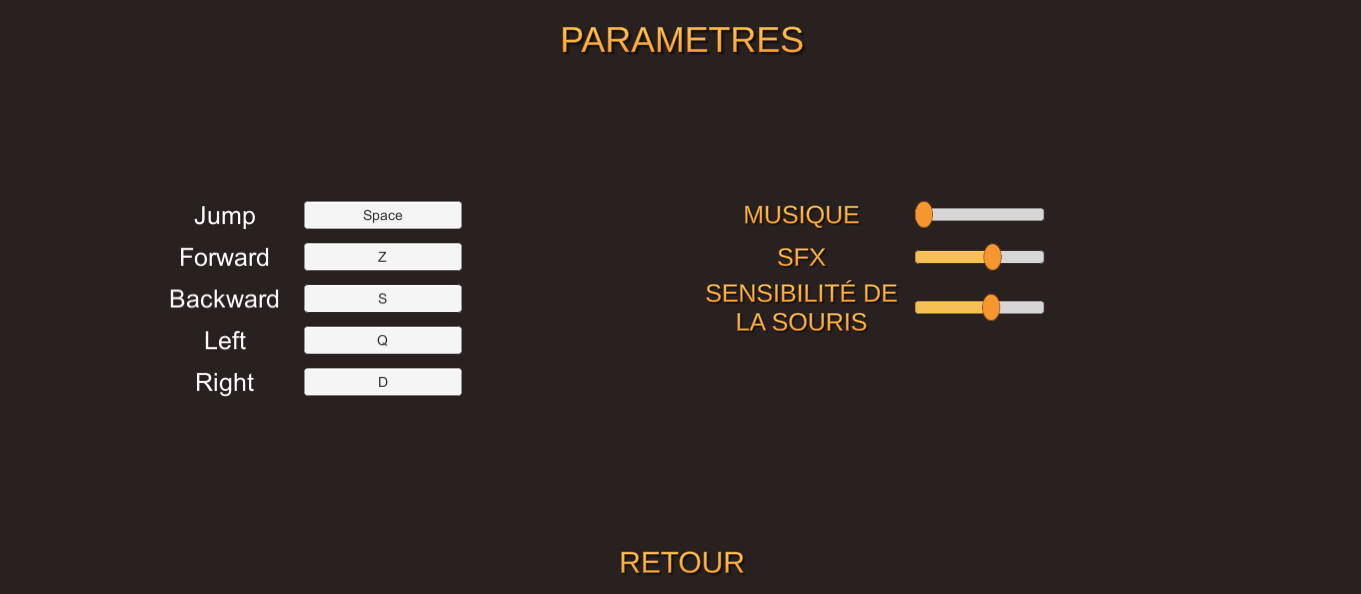
\includegraphics[width=0.8\textwidth]{parametres.png}
    \caption{paramètres écran principal}
\end{figure}

Les trois utilisent des float qui sont utilisé comme coefficient pour le calcul des valeurs correspondantes. La musique et les effets sonores vont de 0 à 1 donc 0 à 100\% du volume. En revanche la plage de valeurs pour la sensibilité de la souris est plus réduite: de 0.1 à 0.8. J'ai limité ces valeurs car une sensibilité de 0 revindrait à ne pas bouger la caméra. Perdre du temps pour revenir aux paramètres car on est allé un peu trop vite peut rapidement mener à une défaite dans ce genre de jeux. Et la limite supérieur est tout à fait arbitraire car je me suis rendu compte que au-delà, la caméra devenait ingérable et l'expérience de jeu en souffrait.

\newpage

Voici une des fonctions de ces paramètres, on remarque qu'elle est assez simple:

\par\vspace{0.2cm}
\begin{lstlisting}
    public void OnMouseSensitivityValueChange(float value)
    {
        mouseSensivity = value;
        PlayerPrefs.SetFloat("mouseSensivity", mouseSensivity);
        PlayerPrefs.Save();
    }
\end{lstlisting}

Elle prends la valeur du slider directement en argument et change la sensibilité de la souris. On sauvegarde ensuite cette valeur pour les prochaines parties.

\paragraph{Salles}
Avec Léandre nous nous sommes répartis la création plus concrète des salles (pour éviter le vert et violet) Nous avons donc utilisé le logiciel Blender pour faire les modèles 3D des différentes salles
Je me suis occupé de faire la salle de croisement, l'impasse et le carrefour.

\subparagraph{La salle de croisement}\hspace{-0.2cm}est assez simple il y a un tableau d'information vide pour l'instant sur le mur libre. Nous y ajouterons sûrement des feuilles. Les trois autres murs ont des portes pour se déplacer dans le labyrinthe.

\begin{figure}[!h]
    \centering
    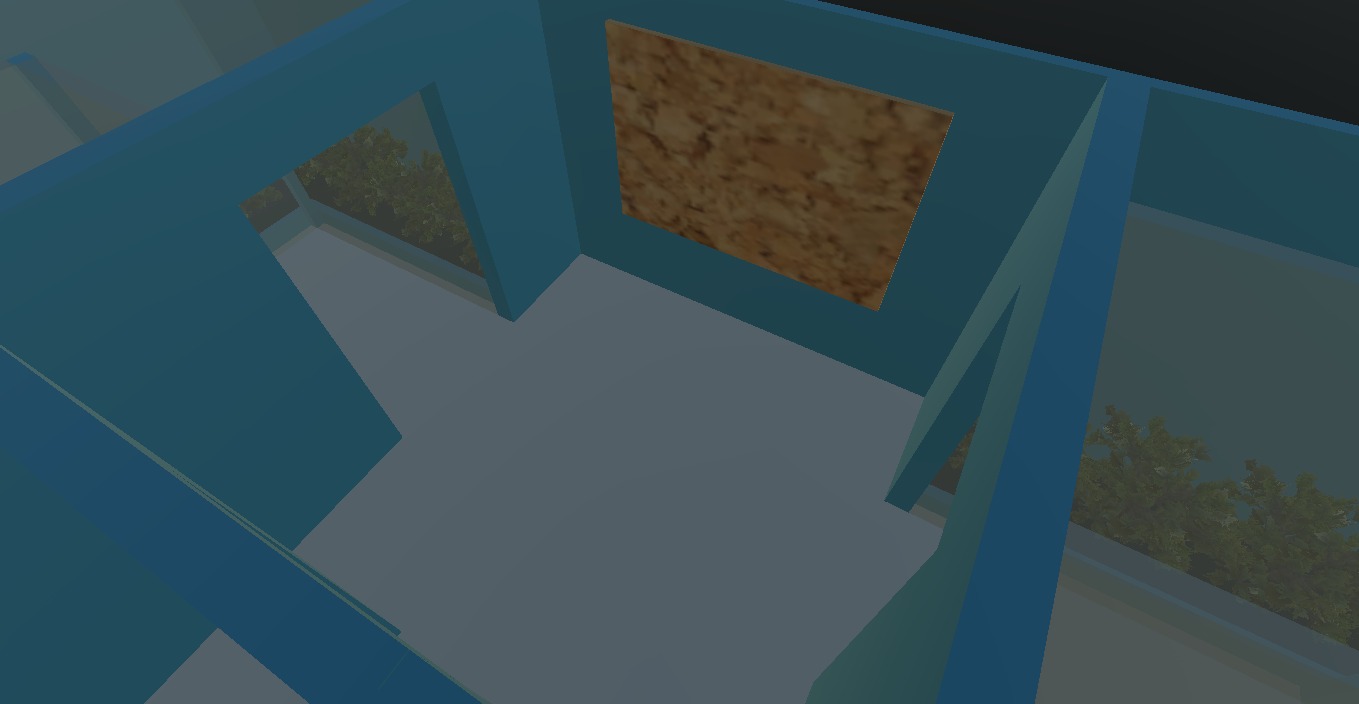
\includegraphics[width=0.8\textwidth]{salle_croisement.png}
    \caption{Salle de croisement}
    \label{salle de croisement}
\end{figure}

\subparagraph{L'impasse}\hspace{-0.2cm}est une salle de stockage/chambre froide nécessaire à toute installation scientifique. Elle comporte une armoire vitrée avec différent fioles de produits d'origines douteuses et d'effets inconnus ainsi que duex armoires blindées dont les explorateurs n'ont malheureusement pas les clés. Un poster orne le mur du fond, montrant la sobriété des développeurs du jeu...

\begin{figure}[!ht]
    \centering
    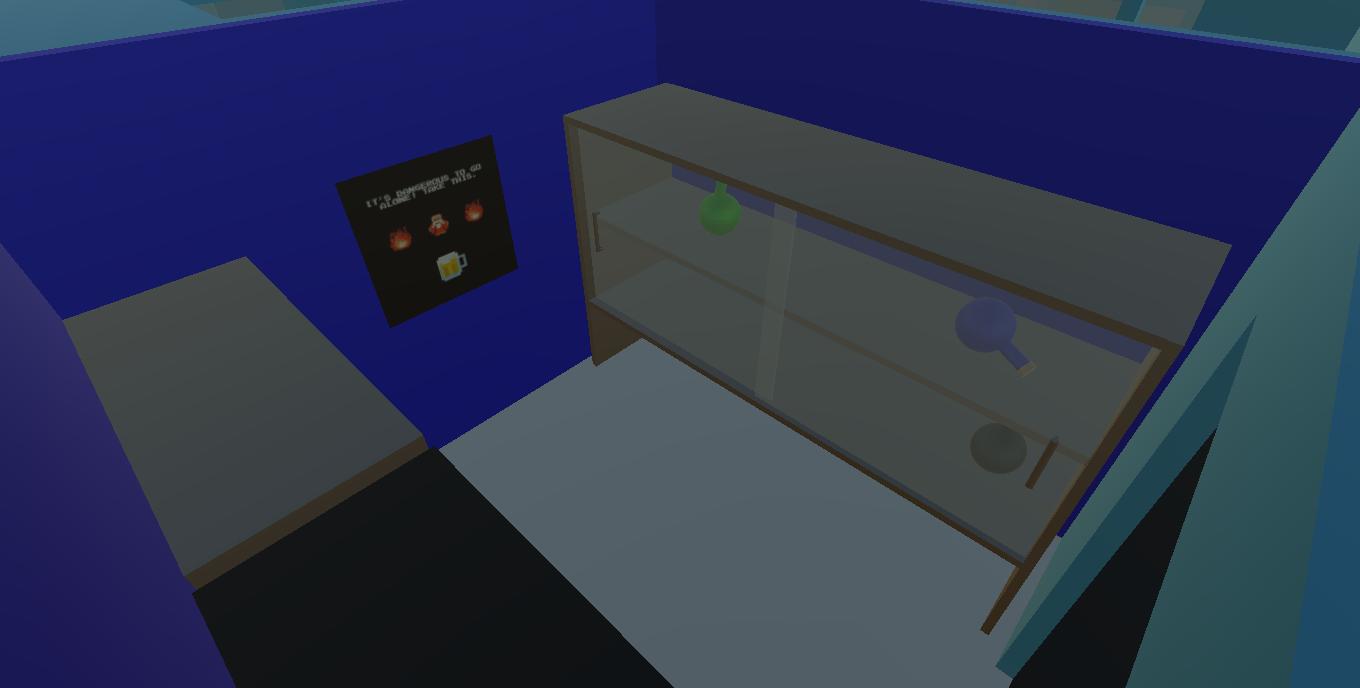
\includegraphics[width=0.8\textwidth]{impasse.png}
    \caption{Impasse}
    \label{Impasse}
\end{figure}

\newpage
\subparagraph{Le carrefour}\hspace{-0.2cm}, bien que rare, apparait sous la forme d'une salle de contrôle avec des écrans (éteints, c'est un laboratoire abandonné quand même), des tableau électriques aux murs et une chaise dans un coin.

\begin{figure}[!ht]
    \centering
    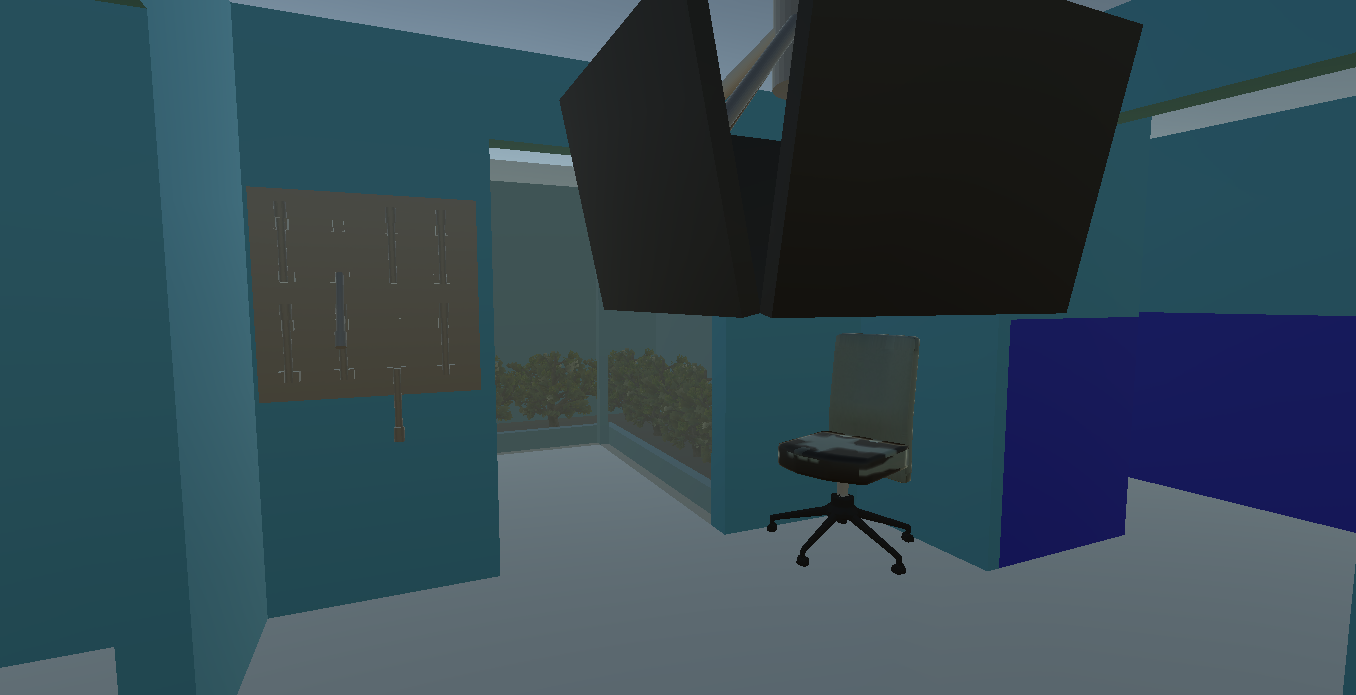
\includegraphics[width=0.8\textwidth]{carrefour.png}
    \caption{Le carrefour du laboratoire}
    \label{carrefour}
\end{figure}

\paragraph{Le site internet}
Je suis responsable de la création du site web de notre groupe. Le header contient notre logo en haut à gauche du site ainsi que le nom du jeu: "Deadly Science". On y retrouve également le menu de navigation du site. Après m'être entretenu avec mes camarades j'ai choisi de faire 5 pages sur le sites:

\begin{itemize}
    \item L'accueil, qui présente notre projet et explique le déroulement du jeu en deux phases: arrivée dans un laboratoire abandonné et infecté par une maladie les joueurs cherchent des sérums capable de les sauver mais insuffisant en nombre. Puis la vengeance du condamné qui veux se venger de ses ex-compagnons.
    \item Le groupe, présentation des membres du groupe avec une photo de chacun.
    \item La galerie contient des photos des différentes salles du laboratoire. J'y ajouterai par la suite des vidéos d'exemples du jeu.
    \item Le codex plaga, pour l'instant vide, expliquera plus en détails le fonctionnement du jeu terminé
    \item Les Documents, vous pouvez y retrouver le cahier des charges le rapport de la première soutenance ainsi que le deuxième.
\end{itemize}{}

%%%%%%%%%%%%%%%%%%%%%% Steve %%%%%%%%%%%%%%%%%%%%%%%%%%%%%%
\newpage
\subsection{Steve}

\paragraph{Réseau}
\subparagraph{Apparition des joueurs}

Comme dans la soutenance précédente, j’ai la charge du projet et je me charge aussi particulièrement du réseau. L'un des plus grands obstacles qu'on a rencontré lors du réseau est l'identification des joueurs. En effet, il serait bien plus plaisant de jouer si chacun des joueurs pouvait apparaître dans un endroit différent du labyrinthe pour premièrement ne pas avoir d'informations concernant l'emplacement des autres joueurs, et deuxièmement pour ne pas savoir notre propre position dans le labyrinthe. Au début, on avait pensé à faire apparaître chacun des joueurs dans un coin du labyrinthe mais cela pourrait donner des informations sur notre emplacement et pourrait nous faciliter la recherche des sérums.

Finalement, on a décidé de les faire apparaître aléatoirement dans le labyrinthe mais de manière que chacun des joueurs apparaissent à un endroit différent. Ils apparaitront dans une cage et lorsque la partie débutera, une trappe en dessous du joueur s'activera et fera tomber les joueurs dans le dédale.

\subparagraph{Distinction du client local des autres clients}

Au premier abord, cela semble très simple mais c'est peut-être l'un des plus grands défis de programmation que j'ai dû relever à ce jour. Plus d'une dizaine d'heures ont été passés juste pour cette tâche.
On a dans un premier temps, pensé à prendre la liste des joueurs affichés dans le menu précédant, puis à chaque joueur lui assigner un identifiant, et pouvoir ensuite les faire apparaître à des coordonnées précises grâce à ces identifiants. Malheureusement, on a été heurté un problème que l’on n’arrivait pas à distinguer le joueur client du reste des joueurs. Malgré qu'il y'ait une variable Player.LocalPlayer (joueur local en français), lorsque que nous avons fait des différents tests, nous nous sommes rapidement rendu compte que le LocalPlayer portait les mêmes informations que tous les joueurs, c'est à dire même UserID (Identifiant d'utilisateur), ActorNumber (Nombre permettant de déterminer le joueur dans une salle spécifique), et même son pseudonyme. 

\newpage
\subparagraph{Gestion des RaiseEvent}

Dans un second temps, on a pensé a utiliser les RaiseEvent (Emetteur d'événements) pour pouvoir les envoyer au MasterClient (l'hôte de la partie), pour qu'il serve de base et puisse traiter les différents messages. Cette solution posait deux problèmes : le premier est qu'on ne puisse pas déterminer l'émetteur du signal. En effet, les RaiseEvent possèdent peu de paramètres, on peut :


\begin{itemize}
\item Soit les envoyer à tout le monde
\item Soit uniquement au MasterClient (il aurait aussi fallu régler le problème que le MasterClient ne s'envoie pas des signaux à lui-même)
\item Soit à tous les autres joueurs (encore une fois, si on veut déterminer le joueur émetteur il faut une liste de tous les joueurs et voir lequel des joueurs n'apparait pas dans la liste, mais comme précédemment cela semble trop complexe). 
\end{itemize}

Mais le second problème et le plus grand, c'est que lorsque qu'on met dans le code d'envoyer le message, tous les joueurs vont envoyer le même message !

\subparagraph{Utilisation des Photon Views}

Et donc à partir de là, malgré de multiples tentatives de gérer les flux entrants des flux sortants, ce fut bien complexe. On a aussi pensé à utiliser les Photon Views (abrégées PV, moyen de reconnaitre facilement par un identifiant un objet contrôlé soit par la scène, c'est à dire l'hôte, soit par le client). Le problème c'est que pour mettre une PV, il faut d'abord un objet sur lequel la mettre. Or on souhaite justement à faire apparaître ce dit objet, qui serait notre joueur.   
On a aussi pensé a utilisé des temps de latence pour envoyer les messages, de manière que s'ils sont envoyés un par un, ils seront bien plus simples à manipuler. Le problème c'est que Photon ne perçoit pas le temps de la même manière que nous le faisons. En effet, même si on essaye de recréer cette latence, Photon va par lui-même gérer cette latence et la partager dans tout le réseau. 

\subparagraph{Utilisation du compte de joueurs dans la salle}

Dans la théorie c'est bien, ça permet à ce qu'un joueur avec une bonne connexion n'ait pas d'avantage comparé à celui qui habite dans la campagne, mais dans la pratique et dans notre cas, ce n'est pas ce que l'on souhaite. Après de très longues recherches sur les bas-fonds d'Internet, passer de forums en forums jusqu'à aller demander aux créateurs de Photon, et l'avis de personnes qui en connaissait bien mieux dans la matière que nous. On a opté pour un système utilisant le compte des joueurs dans la partie, car il semblerait que ce soit l'un des seuls attributs de Photon qui dépend réellement du temps (qui a cliqué en premier, qui a la meilleure connexion etc. ...) Et ça fonctionne bien et c'est le principal !
\newpage
Voici de manière simplifiée comment ça marche:

On regarde le compte de joueurs et s'il l'égal à un on le fait apparaître à la position 1
\begin{lstlisting}
if (PhotonNetwork.CountOfPlayers == 1)
{
            PhotonNetwork.Instantiate(Joueur, Position1, sans_rotation)
}

if (PhotonNetwork.CountOfPlayers == 2)
{
            
}
\end{lstlisting}

Etc... En réalité le code est un peu plus complexe. A la place de faire une succession de conditions imbriquées, on utilise des propriétés du labyrinthe de manière à ce qu'il soit dans une coordonnée aléatoire du labyrinthe mais valide, c'est à dire à la bonne hauteur, pas à l'extérieur, pas dans un mur etc...

\paragraph{Menus}

Pour ajouter de la personnification aux jeu, Léandre et moi avons travaillé encore ensemble pour rendre le gameplay et la jouabilité meilleure. L'une des idées qui furent mises sur la table est que l'hôte de la partie pourrait choisir les dimensions du labyrinthe à partir d’un menu et pourquoi même pour l'avenir un choix de dimension infini en laissant l'hôte taper ses propres coordonnées pour le labyrinthe. 

Pour cela il a fallu créer un menu avec une Scroll List (un tableau déroulant), permettant de sélectionner la dimension que l'on souhaite parmi plusieurs. Lorsqu'on veut sélectionner une dimension qui nous convient, il suffit simplement de cliquer dessus, et le travail est joué ! Un script va interpréter l'action puis l'envoyer à l'autre scène pour que le labyrinthe est connaissance de sa nouvelle dimension. Il a aussi refallu changer l'interface du menu de la salle pour l'hôte de manière qu'il ne puisse pas cliquer ou non sur le bouton "Ready" (prêt en français, vu que ce c'est lui qui détermine quand on commence la partie). Voici un prototype :
\\
\\

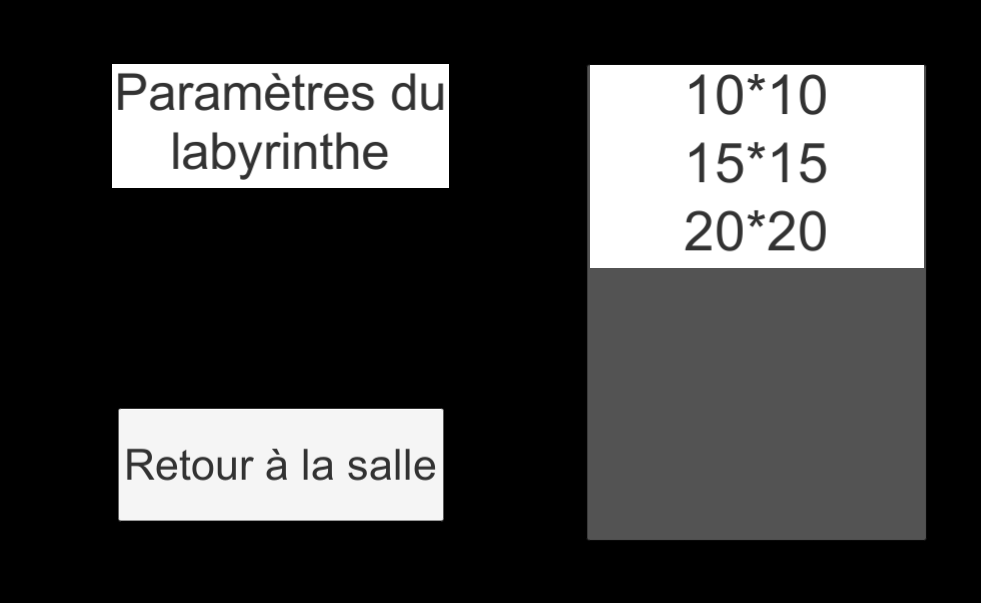
\includegraphics[width=0.9\textwidth]{menustevetaillelabyrinthe.png}\par\vspace{0.75cm}
 
Pour l'instant on a décidé de se contenter de ces trois dimensions car les autres n'étaient pas jouables. En dehors de ça, il a fallu faire les tâches classiques qui sont d'optimiser les scripts, nettoyer les salles des objets de test, repenser les menus pour qu'ils soient plus intuitifs et plus plaisant à regarder...

\newpage
\subsection{Leandre}

Dans ce projet, je suis principalement responsable de la génération aléatoire de la partie ainsi que de la direction artistique. Dans le cadre de cette soutenance, je me suis donc concentré sur la génération des joueurs et des sérums, ainsi que sur la musique et les décors, étant donné que la génération du labyrinthe était déjà en partie terminée, et que la plupart de nos test nécessitent la possibilité de simuler une véritable partie, notamment en ce qui concerne le passage de phase, les passations d'infection, ou encore les fins de partie.

\subparagraph{Génération Aléatoire des Joueurs et des Sérums :}


Afin de ne pas résumer le jeu à une roulette russe, nous avons décidé de faire en sorte que les joueurs et les sérums soient tous sur des cases distinctes, afin d'éviter qu'un joueur ne se retrouve à l'intérieur d'un autre, ou qu'un joueur soit directement guéri dès le début. Mais pour cela, il fallait s'assurer que les coordonnées soient toutes distinctes. Pour ce faire, j'ai commencé à développer une fonction qui générait sept positions aléatoires et distinctes dans le cadre du labyrinthe à partir de sa taille. Cette fonction est ensuite appelée lors de la création du Salon de jeu par le Master, et la liste, ainsi que la taille du labyrinthe, sont envoyées en réseau en tant que variables accessibles à tous. Ainsi, lorsqu'un joueur est généré d'après le code de Steve, il m'a suffi de lui affecter la coordonnée correspondant à son rang pour pouvoir le générer dans une pièce différente des autres joueurs. Quant aux sérums, il fallait qu'ils ne soient générés que par une seule personne. Ce rôle appartient au Master du Salon de jeu, qui, en même temps que son personnage est instancié dans le labyrinthe, génère également les trois autres sérums. On a donc actuellement la possibilité d'apparaître de manière totalement aléatoire dans le labyrinthe lorsque la partie commence, à un emplacement différent des sérums et des autres joueurs. De plus, j'ai également modifié les variables du jeu pour que la taille du Labyrinthe soit décidée par le Master lors de la création du salon. Il ne manque plus qu'à rajouter un bouton pour lui laisser le libre arbitre sur ce paramètre.


\subparagraph{Ambiance sonore :}

Pour travailler sur les musiques du jeu, j'ai utilisé un logiciel de partition nommé MuseScore, qui, en plus d'être gratuit, permet de générer directement une partition complète avec de nombreux instruments, et d'exporter la piste sonore en fichier MIDI. J'ai commencé dans un premier temps à faire plusieurs essais d'ambiance pour le thème de la Recherche de Sérum. Je tenais à rendre l'atmosphère assez stressante. Pour cela, j'ai utilisé un violon qui émet une note à intervalles précis et réguliers, à la manière d'une alarme d'évacuation. J'ai ensuite rajouté une percussion pour renforcer l'ambiance pesante et lourde, tout comme la contrebasse qui se charge du thème. Ensuite, Célian a remixé la piste obtenue, et le résultat est celui que vous pouvez entendre à vos oreilles en lançant une nouvelle partie.

Ensuite, j'ai commencé à faire le thème du Menu Principal. Ici, je tenais à rendre l'atmosphère plutôt pesante et inquiétante. J'ai donc inséré en fond un piano qui répète la même note à la manière d'un tictac d'horloge, accompagné d'un trombone qui se charge de la basse. Enfin, j'ai également composé deux mélodies, l'une pour la victoire, la seconde pour la mort du joueur. Pour la première, j'ai cherché à faire quelque chose d'assez joyeux et léger, tandis que pour l'autre, j'ai utilisé des instruments beaucoup plus graves ainsi que des notes plus longues pour accentuer le sentiment de deuil. Tout comme pour la musique de la recherche de sérums, c'est Célian qui s'est chargé de remixer le tout, en modifiant notamment l'instrumentation. Actuellement, le jeu possède donc quelques musiques originales. Cela dit, ces dernières ne sont encore qu'au stade d'ébauche, et rien ne garantit qu'elles seront encore présentes dans la version finale du jeu.

\subparagraph{Décors :}

L'un des détails les plus importants du jeu, c'est que les joueurs sont dans les souterrains d'un laboratoire, et non dans un dédale quelconque. Avec Yann, nous nous sommes donc entretenus sur les différents types de décor qu'il pourrait y avoir dans le souterrain d'un laboratoire. Nous avons pensé ainsi à des serres, des salles expérimentales, des couloirs avec des extincteurs et des alarmes d'incendie, des salles d'archives, des salles de stockage ou encore des salles de réflexion. En fonction de la pertinence de ses salles, nous les avons répartis par type de salle : impasse, salle à deux issues opposées, à deux issues adjacentes, à trois issues ou encore à quatre issues. D'après mon algorithme de génération de labyrinthe, les salles les plus fréquentes sont celles à deux et à trois issues, puis les impasses, et enfin les salles à quatre issues.

Je me suis ainsi occupé de faire des serres, des couloirs, et des salles d'expérimentation. Pour cela, Yann et moi avons utilisé le logiciel de modélisation tridimensionnelle Blender. Pour faire les serres, associées aux salles à deux issues adjacentes, j'ai décidé de placer des vitres et d'insérer derrière des plants de plantations diverses, ce qui fait que les joueurs peuvent se déplacer dans un espace entre deux vitres, à l'image d'un couloir classique. Pour les salles à deux issues opposées, nous avons opté pour une salle d'expérimentation. Ici, les murs ne sont pas physiques, mais reposent plutôt sur la paillasse d'un côté et une hotte et une armoire de l'autre. Enfin, concernant les couloirs banals, j'ai opté pour une version des salles à trois issues en m'inspirant des murs d'hôpitaux. Les préfabriqués ont ensuite été inséré dans Unity, et je me suis chargé de remplacer les anciens préfabriqués (qui étaient vert fluo et mauve vif) par ces nouveaux, en faisant attention à ce que tout soit identique, notamment la possibilité de mise en réseau par Photon et les possibilités de déplacement. J'ai également dû redéfinir de nouveaux matériaux, étant donné que je n'ai pas trouvé comment conserver les matériaux présents sur Blender à Unity. J'ai ensuite aidé Yann à insérer les préfabriqués qu'il avait conçu dans le jeu. Actuellement, toutes les salles sont regardables sans déclencher d'hémorragie visuelle, ce qui est déjà un bon début. Mais nous n'avons pas encore terminé, vu qu'il nous reste encore à rajouter quelques détails pour renforcer la cohérence des décors, comme par exemple des tabourets, des tâches, des boulettes de papier ou encore du matériel expérimental.

J'ai également modifié l'apparence des sérums avec Blender, afin de les rendre plus jolis : auparavant, ils ressemblaient à des cubes pour enfant, maintenant, ils ressemblent beaucoup plus à des fioles expérimentales. Enfin, l'un des derniers détails concernant la décoration du jeu concerne un problème que Yann et moi avons rencontré avec les salles électriques, qui ont quatre issues : en effet, Yann avait placé au centre quatre écrans. Or, les sérums apparaissant au centre de la pièce, si un sérum apparaissait dans ce type de salle, il restait inaccessible aux joueurs. Nous avons donc opté pour la suppression d'un des quatre écrans, de manière à laisser une ouverture pour le sérum. Cette configuration oblige ainsi les joueurs à se déplacer à un endroit précis de la pièce, au lieu de courir bêtement d'un bout à l'autre. Les salles électriques sont donc les salles les plus difficiles pour la collecte des sérums. Heureusement, il s'agit également des salles les plus rares.

\par\vspace{0.5cm}
\begin{figure}[!ht]
    \centering
    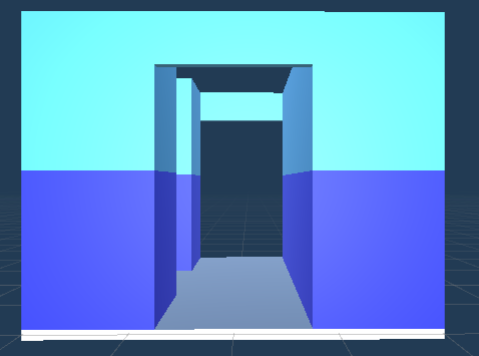
\includegraphics[width=0.5\textwidth]{Bifurc Bas.PNG}
    \caption{Bifurcation - 1}
    \label{Bifurcation - 1}
\end{figure}{}
\par\vspace{0.5cm}
\begin{figure}[!ht]
    \centering
    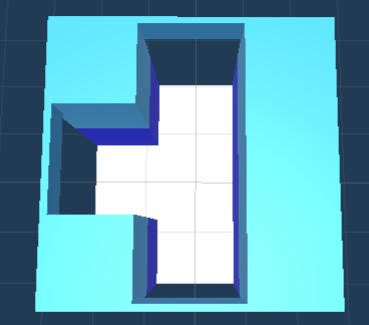
\includegraphics[width=0.5\textwidth]{Bifurc Haut.PNG}
    \caption{Bifurcation - 2}
    \label{Bifurcation - 2}
\end{figure}{}
\par\vspace{0.5cm}
\begin{figure}[!ht]
    \centering
    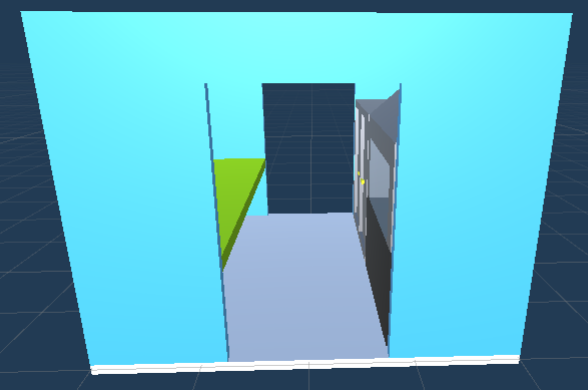
\includegraphics[width=0.5\textwidth]{Droit Bas.PNG}
    \caption{Couloir droit - 1}
    \label{Couloir droit - 1}
\end{figure}{}
\par\vspace{0.5cm}
\begin{figure}[!ht]
    \centering
    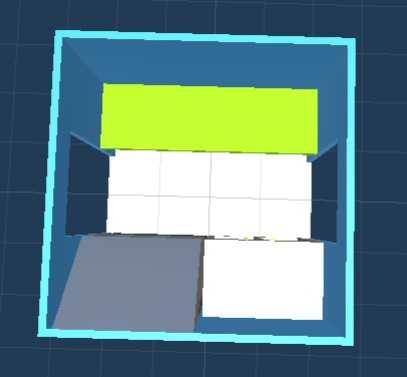
\includegraphics[width=0.5\textwidth]{Droit Haut.PNG}
    \caption{Couloir droit - 2}
    \label{Couloir droit - 2}
\end{figure}{}
\par\vspace{0.5cm}
\begin{figure}[!ht]
    \centering
    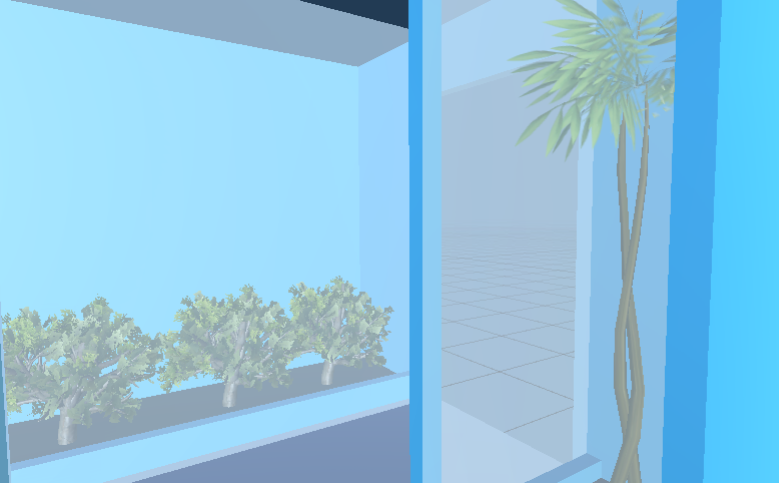
\includegraphics[width=0.5\textwidth]{Tournant Bas.PNG}
    \caption{Couloir tournant - 1}
    \label{Couloir tournant - 1}
\end{figure}{}
\par\vspace{0.5cm}
\begin{figure}[!ht]
    \centering
    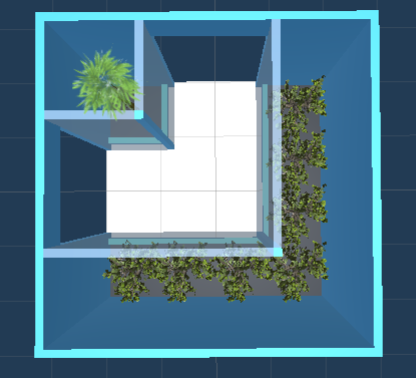
\includegraphics[width=0.5\textwidth]{Tournant Haut.PNG}
    \caption{Couloir tournant - 2}
    \label{Couloir tournant - 2}
\end{figure}{}

\subparagraph{Plafonds :}

Actuellement, lorsque les joueurs sont instanciés, ils se retrouvent directement dans la salle du dédale où ils commencent. Mais dans le jeu final, ils seront auparavant dans une salle au rez-de-chaussée, sur une trappe qui s'ouvrira pour les faire descendre dans les souterrains. Pour préparer le terrain, j'ai donc commencé à mettre au point les plafonds, qui sont présents dans chaque salle où ne commence pas un joueur. L'avantage est que cela permet de vérifier que les quatres joueurs sont bient à des coordonnées différentes au début, et aussi de vérifier qu'ils sont bien instanciés à l'emplacement qu'il leur était prévu (en regardant si la salle où ils se trouvent a un plafond).
Il me restera à rajouter dans les plafonds actuels des lampes pour éclairer les souterrains du laboratoire, ainsi qu'à m'accorder avec Yann pour produire les "salles d'attente".

\par\vspace{0.5cm}
\begin{figure}[!ht]
    \centering
    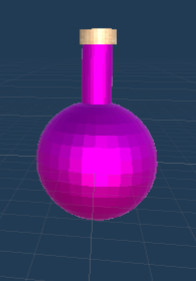
\includegraphics[width=0.5\textwidth]{Fioles.PNG}
    \caption{Fioles}
    \label{Fioles}
\end{figure}{}

\newpage
\section{Conclusion}

En ce qui concerne la prochaine soutenance, le jeu devrait être à peu de choses près fini. D'ici là, il nous reste encore à paufiner les décors et les musiques, à créer les "salles d'attente" pour la génération des joueurs, améliorer la seconde phase, compléter le site en y incluant également le lien de téléchargement du jeu, rendre les menus plus fluides et ergonomiques, et également mettre au point un système permettant d'installer le jeu et de le désinstaller. Autrement dit, il nous reste encore du pain sur la planche, mais ce devrait être largement faisable dans les délais imposés pour le Projet S2.

\emph{If you knew time as well as I do, you would play Deadly Science.}

%%%%%%%%%%%%%%% TODO : Annexes


\end{document}



